\chapter{Max Energy}\label{chapter:max-energy}

Let $\mathcal{C}$ a oriented curve in the plane. We center disks $B_i$ and $B_o$ of radius $R+\epsilon$ with centers aligned with the normal direction of the curve at some point $p \in \mathcal{C}$. Moreover, the distance from disks center to $p$ equals to $R$.

\begin{figure}[h!]\label{fig:r-separated-disks}
\center
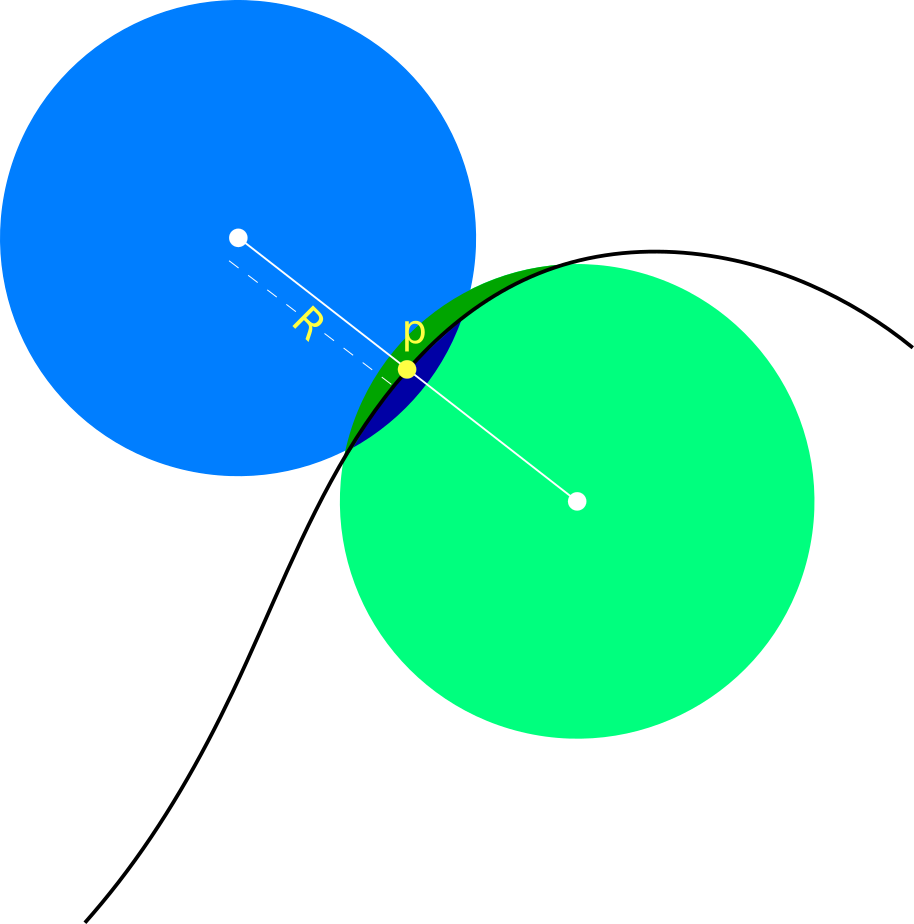
\includegraphics[scale=0.35]{figures/max-energy/r-separated-disks.png}
\caption{disks of radius $R+\epsilon$ distant $R$ units from $p\in \mathcal{C}$ in the normal direction.}
\end{figure}

%-2*sqrt(2)*pi*E^(3/2)*R^(9/2)*k^2 + 2*pi^2*R^4 + 71/210*sqrt(2)*pi*E^(7/2)*sqrt(R) - 28/15*sqrt(2)*pi*E^(5/2)*R^(3/2) - 16/3*sqrt(2)*pi*E^(3/2)*R^(5/2) + 224/45*E^4 + 64/9*E^3*R

Let $\theta_o (\theta_i)$ to denote the intersection of $B_o(B_i)$ with the inner(outer) region of the curve. We define the function $E:\mathcal{C}\rightarrow \mathbb{R}$ as

\begin{align*}
	g(\epsilon,p) &= \big( \pi (R+\epsilon)^2 - \Theta_o(p)\big)^2 + \big(\pi (R+\epsilon)^2 - \Theta_i(p) )^2\\
		 &= g_o(\epsilon,p) + g_i(\epsilon,p)
\end{align*}

\begin{claim}{R-separated disks curvature}\label{claim:r-separated-disks}
 Let $\mathcal{C} \in \mathbb{R}^2$ be a curve such that for a point $p \in \mathcal{C}$ its curvature equals to $\kappa$. For sufficiently small values of $\epsilon$ and $\kappa$, we can approximate $g$ by

\begin{align*}
g(\epsilon,p) \approx &-2 \sqrt{2}\pi \epsilon^{3/2}R^{9/2}\kappa^2 + 2\pi^2R^4 + 8\pi^2\epsilon R^3\\
 &- \frac{16}{3}\sqrt{2}\pi\epsilon^{3/2}R^{5/2} + 12\pi^2\epsilon^2R^2 - \frac{188}{15}\sqrt{2}\pi\epsilon^{5/2}R^{3/2} \\ 
 &+ \frac{8}{9}\big(9\pi^2 +8\big)\epsilon^3R - \frac{611}{70}\sqrt{2}\pi\epsilon^{7/2}\sqrt{R} + \frac{2}{45}\big(45\pi^2 + 112\big)\epsilon^4
\end{align*} 
\end{claim}


\begin{proof} The curvature of a parabola $ax^2 + bx +c$ is given by

\begin{align*}
	\kappa(x) = \frac{2a}{\big(1+(2ax+b)^2\big)^{3/2}}
\end{align*}

Therefore, the parabola $\frac{\kappa}{2}x^2$ has curvature $\kappa$ at $x=0$. We are going to use this parabola to approximate the curve around a point $p \in \mathcal{C}$.

We proceed by computing the intersection area $\theta_o$.


\begin{figure}[h!]\label{fig:parabola-approx-ex}
\center
	\subfloat[\label{}]{%
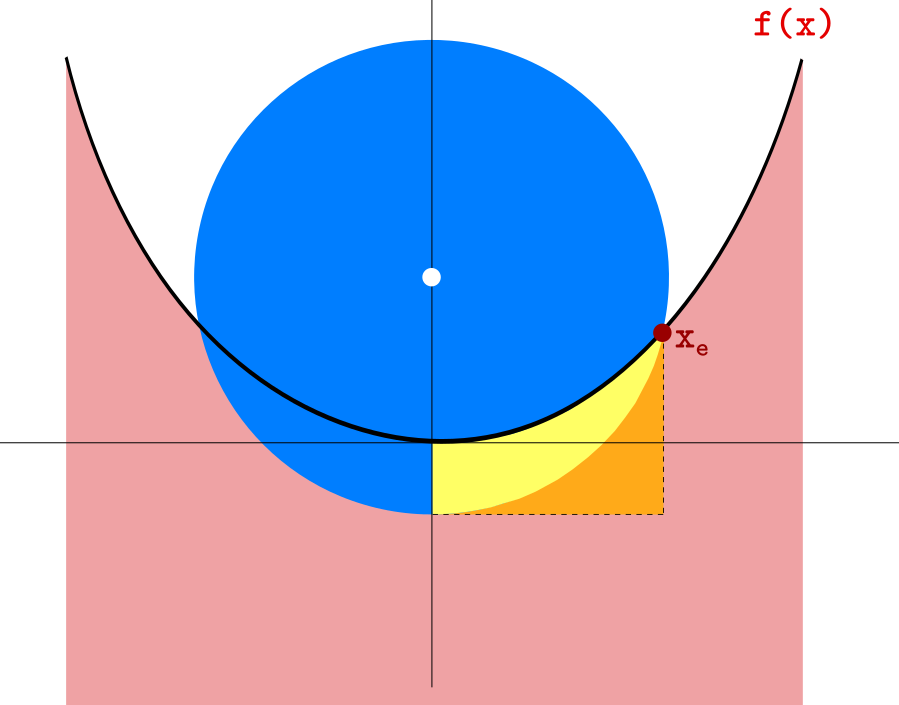
\includegraphics[scale=0.35]{figures/max-energy/parabola-approx-1.png}
	}\hspace{20pt}%
	\subfloat[\label{}]{%
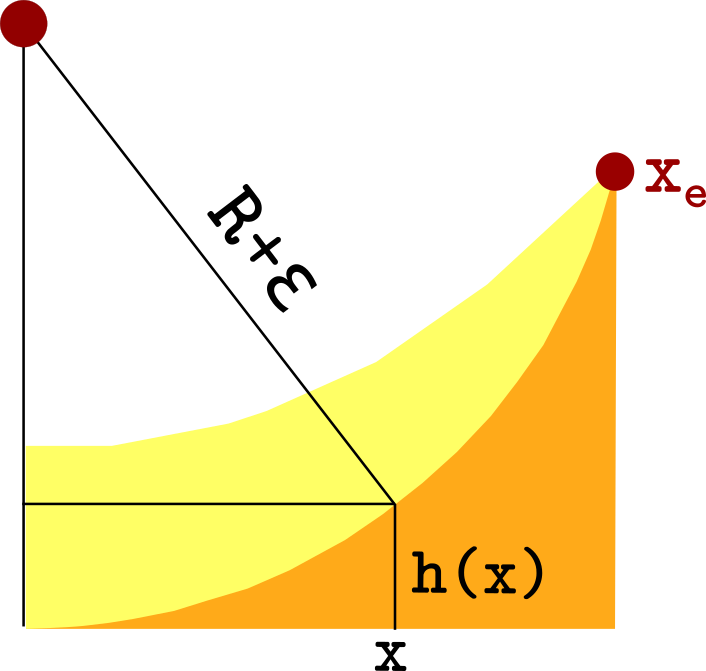
\includegraphics[scale=0.35]{figures/max-energy/parabola-approx-2.png}
	}
\caption{The yellow area corresponds to $\theta_o$ and it equals the area under the parabola from $x=0$ until $x=x_o$ minus the orange area.}
\end{figure}

\begin{align*}
	h(x) &= R+\epsilon - \sqrt{ (R+\epsilon)^2 - x^2}\\
	\theta_o &= 2\int_0^{x_o}{f(x) + \epsilon - h(x)}\\
\end{align*}

To compute the intersection point $x_o$ of the parabola with the disc, we use again pythagoras' theorem.

\begin{align*}
	(R+\epsilon)^2 &= (R-\frac{\kappa}{2}x_o^2)^2 + x_o^2\\
	0 &= \frac{\kappa^2}{4}x_o^4 + (1-R\kappa)x_o^2 + R^2 - (R+\epsilon)^2
\end{align*}

By setting $z_o=x_o^2$

\begin{align*}
\Delta_o &= (1-R\kappa)^2 + \kappa^2(2R\epsilon + \epsilon^2)\\
z_o &= \frac{2}{\kappa^2}(R\kappa-1 + \sqrt{\Delta_o})\\
x_o &= \frac{\sqrt{2}}{\kappa}\sqrt{R\kappa-1+\sqrt{\Delta_o}}
\end{align*}

We proceed similarly for the inner disk.


\begin{figure}[h!]\label{fig:parabola-approx-in}
\center
	\subfloat[\label{}]{%
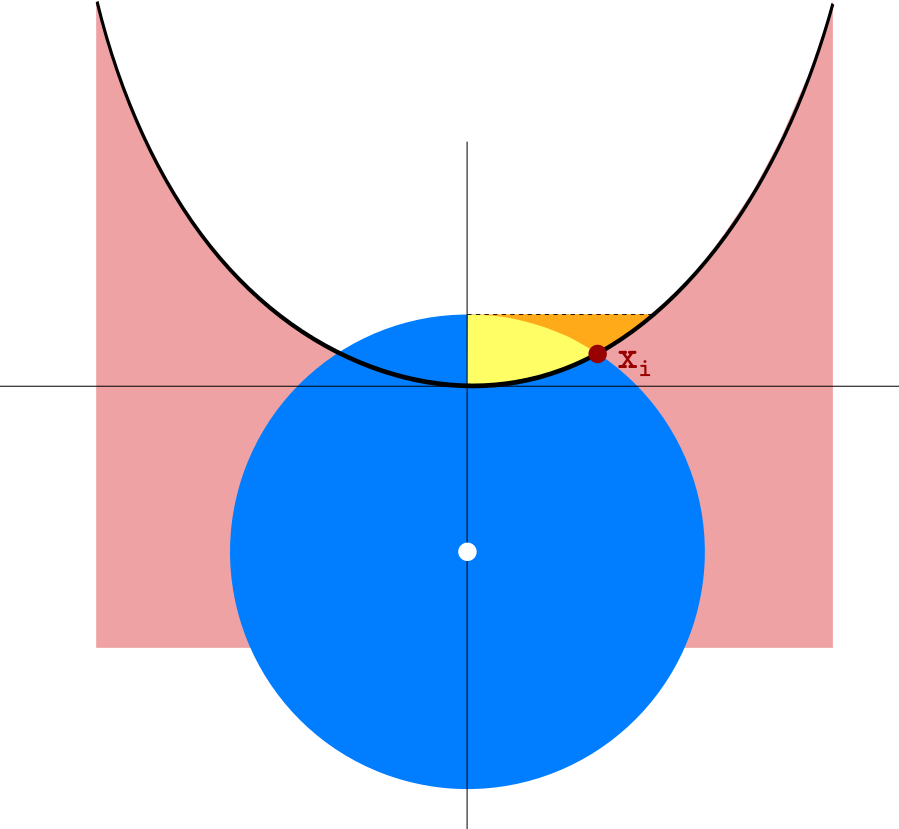
\includegraphics[scale=0.35]{figures/max-energy/parabola-approx-3.png}
	}\hspace{15pt}%
	\subfloat[\label{}]{%
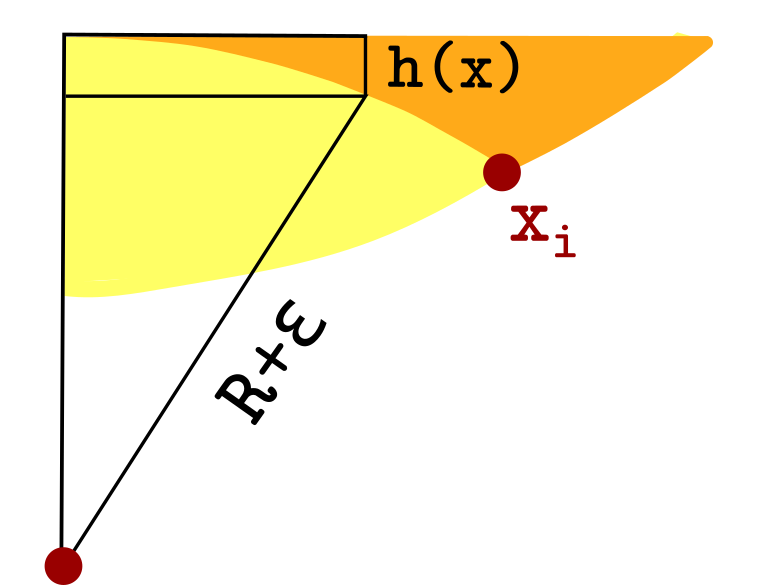
\includegraphics[scale=0.35]{figures/max-energy/parabola-approx-4.png}
	}
\caption{The yellow area corresponds to $\theta_i$ and it equals the area between the parabola and the disc from $x=0$ until $x=x_i$.}
\end{figure}

\begin{align*}
	\theta_i &= 2\int_{0}^{x_i}{\epsilon - f(x) - h(x)}	\end{align*}

The intersection point $x_i$ between the parabola and the inner disk is given by
	
\begin{align*}
	(R+\epsilon)^2 &= (R+\frac{\kappa}{2}x_o^2)^2 + x_i^2\\
	0 &= \frac{\kappa^2}{4}x_i^4 + (1+R\kappa)x_i^2 + R^2 - (R+\epsilon)^2	\\
\Delta_i &= (1+R\kappa)^2 + \kappa^2(2R\epsilon + \epsilon^2)\\
x_i &= \frac{\sqrt{2}}{\kappa}\sqrt{-R\kappa-1+\sqrt{\Delta_i}}.
\end{align*}

The claimed approximation is obtained by expanding $g$ with its  4th order Taylor series around $\kappa=0,\epsilon=0$.
\end{proof}

\section{Curve evolution process}

Given a closed oriented curve $\mathcal{C}$, we define the optimization region $O$ as the band of size $\epsilon /2$ around $\mathcal{C}$. For a given radius $R$, we define the ring $\mathcal{R}$ as

\begin{align*}
	x \in \mathcal{R} \implies \min_{p \in \mathcal{C}} d(x,p) = R.
\end{align*}

The ring is composed of two connected components, denoted here as $C_{inn}$ and $C_{out}$ accordingly with the curve orientation.


\begin{figure}[h!]\label{fig:integral}
\center
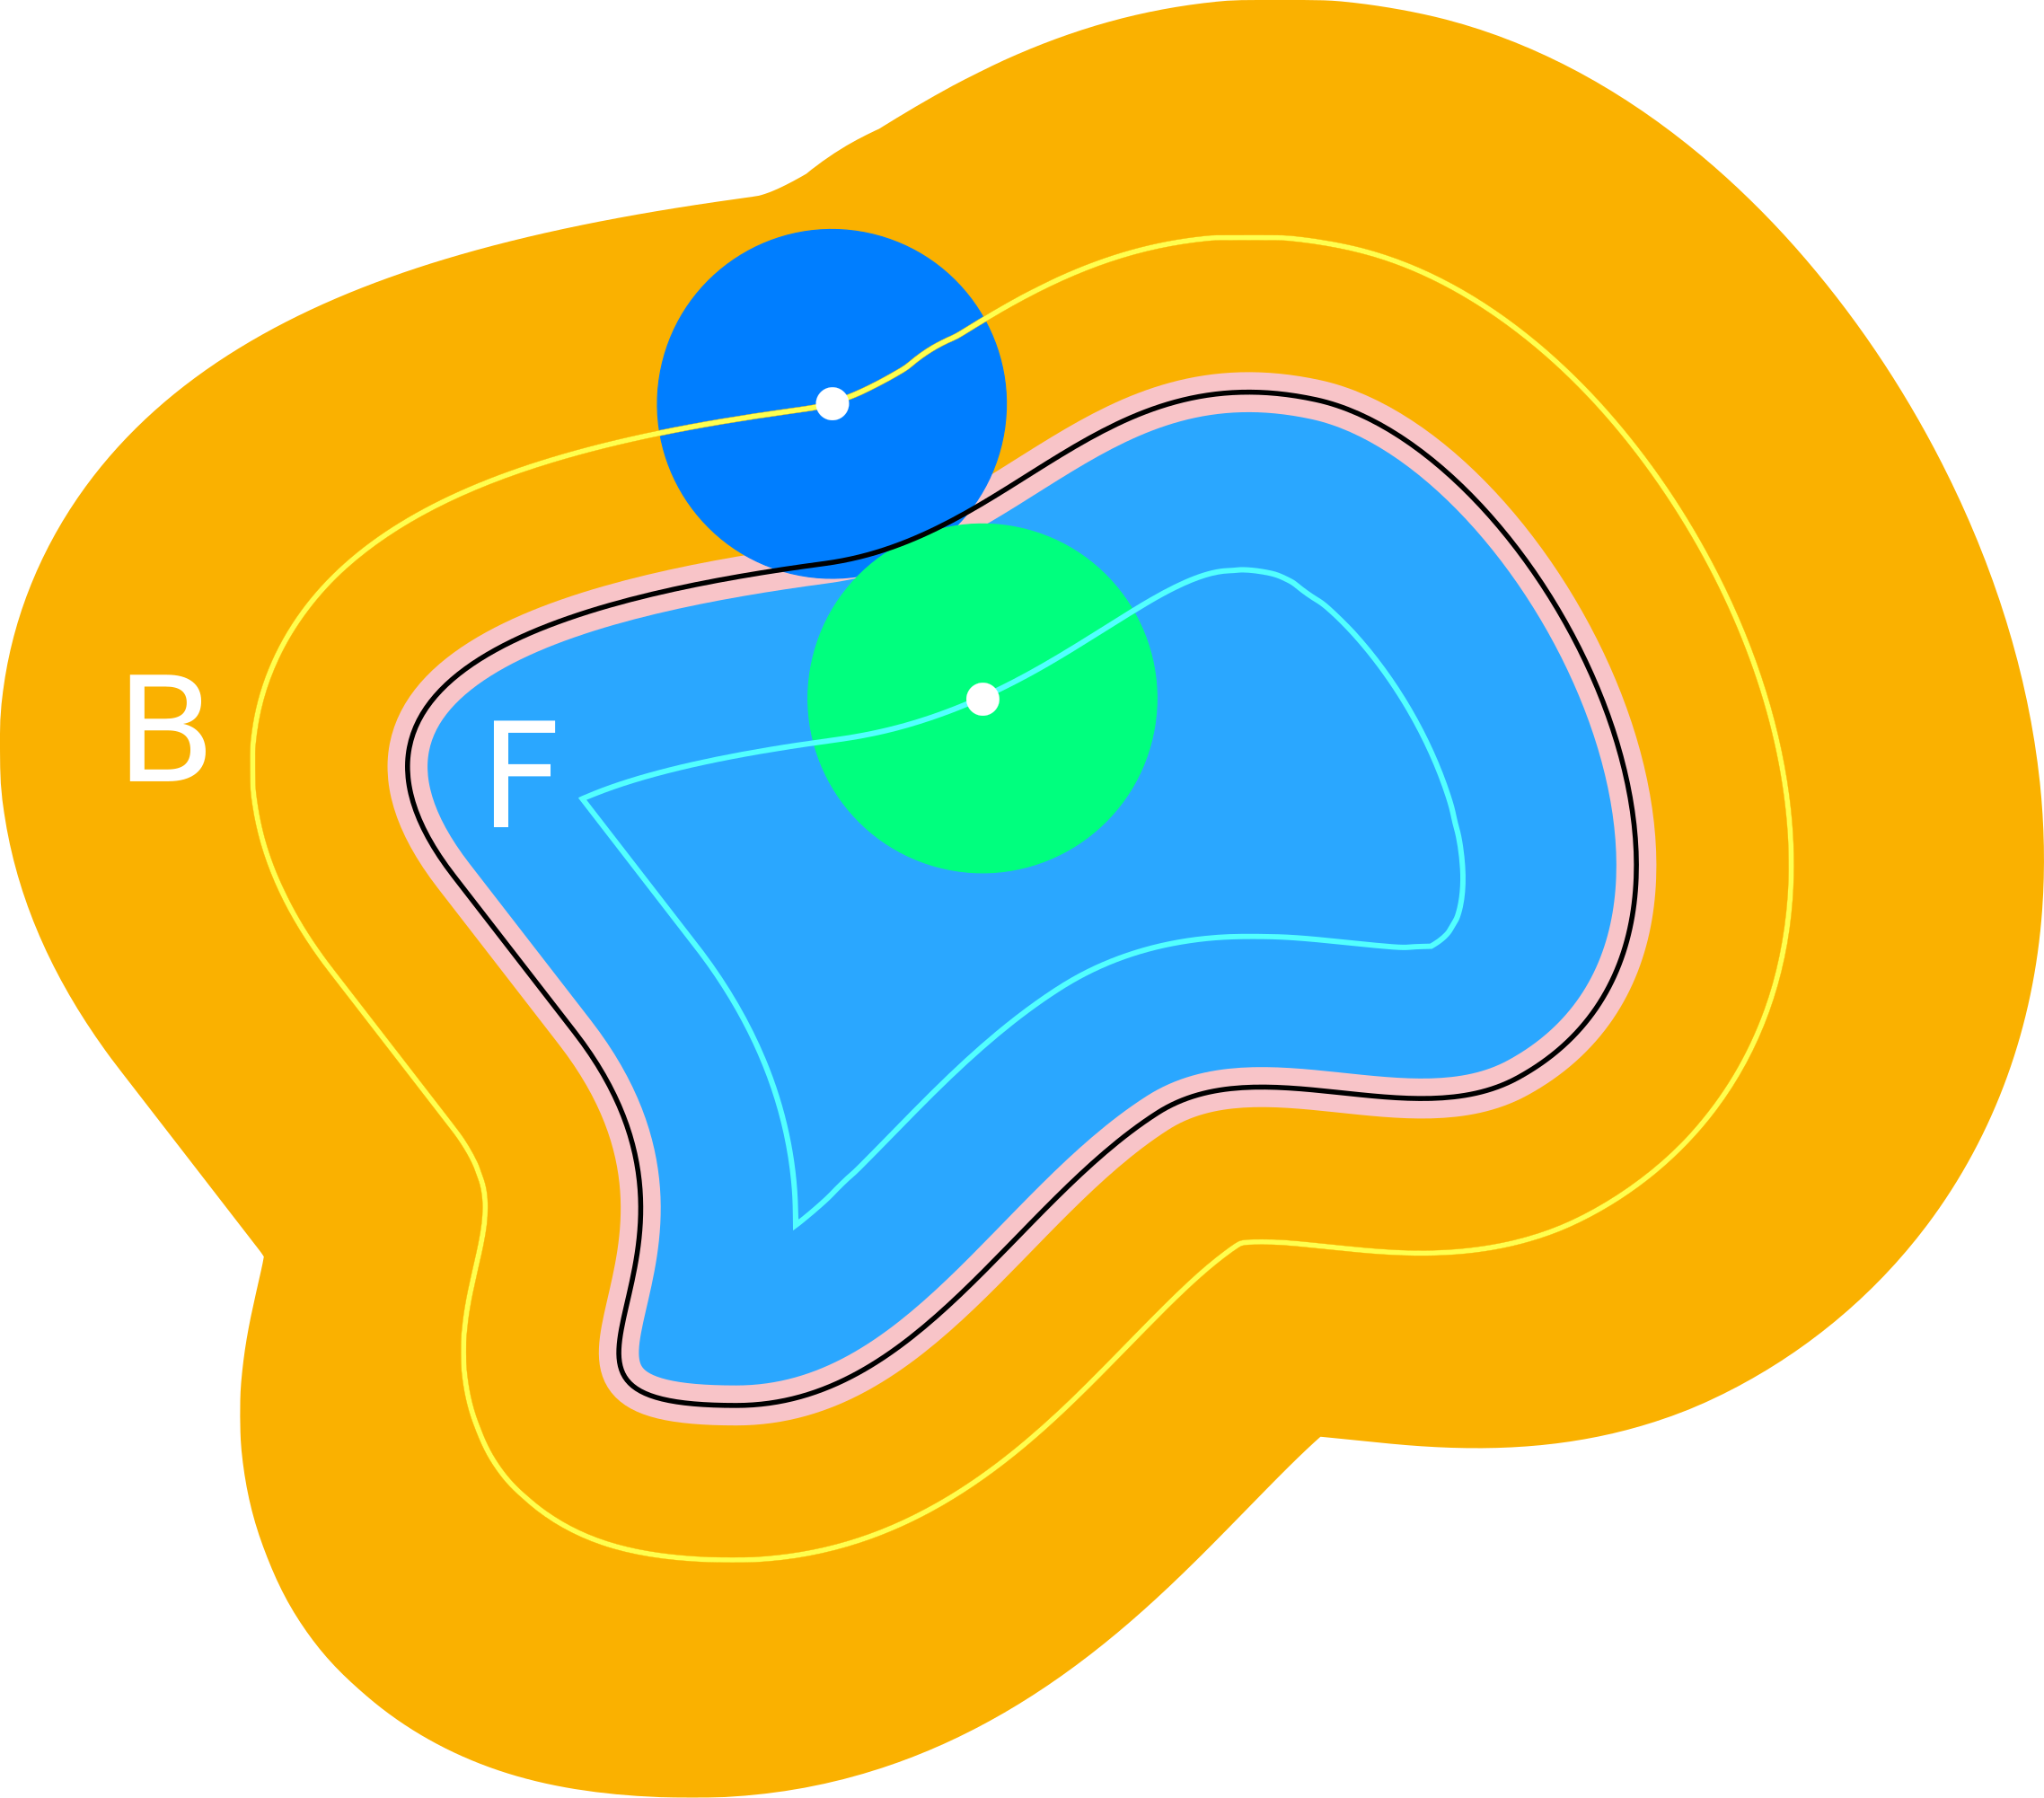
\includegraphics[scale=0.25]{figures/max-energy/integral-2.png}
\caption{The estimation balls are evaluated along the inner and outer curves.}
\end{figure}


We evolve a curve evolution process in which at every step the following optimization process is solved

\begin{align}\label{eq:max-energy}
	\max_{x \in O}{E} &= \max_{x \in O} \sum_{p \in \mathcal{C}_{out}}{g_o} + \sum_{p \in \mathcal{C}_{inn}}{g_i}\\\nonumber 
	&=\sum_{p \in \mathcal{C}_{out}}{ \big( \pi R^2 - F_p - \sum_{x \in O_p}{x}\big)^2} + \sum_{p \in \mathcal{C}_{inn}}{ \big( F_p + \sum_{x \in O_p}{x}\big)^2}\\\nonumber
	&= \sum_{p \in \mathcal{C}_{out}}{ (1 - 2\pi R^2 + 2F_p) \sum_{x \in O_p}{x} + \sum_{ \substack{ x_j,x_k \in O_p \\ j < k}}{2x_jx_k}}\\\nonumber
	&+ \sum_{p \in \mathcal{C}_{inn}}{(2F_p + 1)\sum_{x \in O_p}{x} + \sum_{\substack{ x_j,x_k \in O_p \\ j < k}}{2x_jx_k}}	
\end{align}


\section{Optimization}

Let $\mathfrak{B}=\{0,1\}$. We define $F:\mathfrak{B}^n\rightarrow \mathbb{R}^n$ as a pseudo-boolean function. The function $F$ can be expressed in the form of a multivariate polynomial and its degree is exactly the same of its polynomial, namely, the degree of the monomial with highest degree.

\begin{claim}{Degree-2 reduction}
	A pseudo-boolean function $F$ of any degree can be rewritten as a degree-2 pseudo-boolean function of the form.	
	
\begin{align}\label{eq:pbf-polynomial-form}
	F(X) = \sum_{1\leq i\leq n}{a_ix_i} + \sum_{1 \leq i < j \leq n}{a_{ij}x_ix_j}	
\end{align}	
	
\end{claim}

Sometimes, we may prefer to write $F$ using its literals. A variable $x_i$ possess literals $x_i$ and $\overline{x_i}$ representing the values $1$ and $0$, respectively. The expression \eqref{eq:pbf-polynomial-form} is transformed in:

\begin{align}
	F(X) = \sum_{1\leq i\leq n}{E_i(0) + E_i(1)} + \sum_{1 \leq i < j \leq n}{E_{ij}(0,0) + E_{ij}(0,1) + E_{ij}(1,0) + E_{ij}(1,1)}
\end{align}


\begin{claim}{Submodular} \label{claim:submodular}
 We say that $F$ is submodular if and only if 
 
 \begin{align*}
	E_{ij}(0,0) + E_{ij}(1,1) \leq E_{ij}(0,1) + E_{ij}(1,0).
 \end{align*}
\end{claim}

We say that $F$ is supermodular otherwise. Submodular (supermodular) functions can be efficiently minimized (maximized).

%\textbf{Observation:} One may lead to believe that $F$ in its polynomial form and $a_{ij}\leq0, \forall i,j$ can be solved by a greedy algorithm on the unary terms $a_i$. That is not true, as the function below illustrates
%
%\begin{align*}
%	-10x_1 + 2x_2 + 2x_3 -x_1x_2 -x_1x_3 -10x_2x_3
%\end{align*}
%
%The greedy solution would return $f(1,0,0)=-10$, while the correct minimum is $f(1,1,1)=-18$.

\begin{claim}{Optimization of $E$}
	Function $E$ is supermodular.
\end{claim}

\begin{proof}
	From equation \eqref{eq:max-energy} we observe that all pairwise coefficients are positive. Then, by claim \ref{claim:submodular}, the function is supermodular.
\end{proof}


\section{Open issues}

\begin{enumerate}
	\item{In practice, how accurate can be an estimator for curvature based on the Taylor expansion of $g$? In particular, for each values of $\kappa$ with respect to $\epsilon$ the expansion is a good approximation?}
	\item{The analytic results were obtained in a local framework. How can we extend this interpretation for the integral computation that we evaluated in the flow?}
	\item{The inner and outer curves have different perimeters. How can we set their weights properly?}
\end{enumerate}


\section{Experiments}

\subsection{Experiment 1}
\textbf{Hypothesis:} The flow advances from interior if outer ball doesn't touch pixels that are touched by the inner ball.


\textbf{Experiment description:} Execute the flow over a curvy face where we know curvature elsewhere (e.g. the bean shape). If we use a ball of radius smaller than the reach, in no ocassion the inner(outer) ball won't touch any pixels. Therefore, by the hypothesis, the shape should not evolve.


\textbf{Result:} The hypothesis demonstrated wrong, as the shape evolves anyway. But inspire us to do a second experiment.

\subsection{Experiment 2}

\textbf{Hypothesis:} The flow advances towards the outer shape at $p$ if $G_i(p) > G_o(p)$.


\textbf{Definitions:} Define the hitting inner(outer) curve of some pixel $p$ in the digital curve $H_i(p)$($H_o(p)$) as the set of points  $q$ in the inner(outer) curve in which a ball of radius $r$ centered at $q$ touches $p$. For a point $q \in H_i(p)$, define its gain as $G_{p}(q) = 2DA - D^2$, where $A$ is the disk area and $D$ its deficit. For the inner curve, its deficit is the disk area not covering the shape interior. We define the gain of $p$ as $G_i(p) = \sum_{q \in H_i(p)} G_p(q)$, and we do similarly for $G_o(p)$. 


\textbf{Experiment description:} A possible way is to derive the positive ot negative conclusion from analytical development. Otherwise, one can code a flow that works as its proposed here and then compare the results.


\textbf{Result:} Not tested yet.


\subsection{Experiment 3}

\textbf{Hypothesis:} The inner and outer perimeter differences is the main responsible for the flow evolution.

\textbf{Experiment description:} Evolve the flow in such a way that outer and inner perimeters have the same weight. For example, set inner ball coefficient one and outer  ball coeficient as $L_{inn}/L_{out}$.

\textbf{Result:} The flow presents interesting behaviour. Regions of negative curvature always expand, but regions of positive curvature may decrease or increase, depending of its proximity with the closest positive curvature region. For example, the upper convex parts of the bean shape shrinks, while its bottom convex part dilates.


\subsection{Experiment 4}

\textbf{Hypothesis:} If curvature is negative, the energy is better of by maximizing the inner ball. If curvature is positive, the energy is  better of by maximizing the outer ball.


\textbf{Experiment description:}


\textbf{Result:} Experiment 3 demonstrated that this hypothesis is false.



\subsection{Experiment 5}

\textbf{Hypothesis:} Evolution for the flower with parameters $h=0.5,r=5,l=-1$ leads to iteration with disconnected components. Those components appear at regions of local flatness. Is that an issue caused by the perimeter weigth in inner and outer curves?


\textbf{Experiment description:}


\textbf{Result:}